%%%%%%%%%%%%%%%%%%%%%%%%%%%%%%%%%%%%%%%%%%%%%%%%%%%%%%%%%%%%%%%%%%%%%%%%%%%%%%%%
%2345678901234567890123456789012345678901234567890123456789012345678901234567890
%        1         2         3         4         5         6         7         8

\documentclass[letterpaper, 10 pt, conference]{ieeeconf}  % Comment this line out if you need a4paper

%\documentclass[a4paper, 10pt, conference]{ieeeconf}      % Use this line for a4 paper

\IEEEoverridecommandlockouts                              % This command is only needed if 
                                                          % you want to use the \thanks command

\overrideIEEEmargins                                      % Needed to meet printer requirements.

% See the \addtolength command later in the file to balance the column lengths
% on the last page of the document

% The following packages can be found on http:\\www.ctan.org
%\usepackage{graphics} % for pdf, bitmapped graphics files
%\usepackage{epsfig} % for postscript graphics files
%\usepackage{mathptmx} % assumes new font selection scheme installed
%\usepackage{times} % assumes new font selection scheme installed
%\usepackage{amsmath} % assumes amsmath package installed
%\usepackage{amssymb}  % assumes amsmath package installed
\usepackage{graphicx}

%\title{\LARGE \bf Elbow Joint Angle Estimation Through The Measurement of Surface Electromyography
%}
% * <aforner@usp.br> 2018-01-28T08:34:32.702Z:
%
% ^.
\title{\LARGE \bf Elbow Joint Angle Estimation from Surface Electromyography Using Hammerstein-Wiener Models
}

\author{Leonardo Fischi Sommer and Arturo Forner-Cordero% <-this % stops a space
\thanks{Leonardo Fischi Sommer and Arturo Forner-Cordero are with the Biomechatronics Laboratory, Escola Politecnica of the University of Sao Paulo, Avda Prof Mello Moraes, 2231, Sao Paulo, Brazil {\tt\small leonardo.sommer@usp.br, aforner@usp.br}}
}
\begin{document}



\maketitle
\thispagestyle{empty}
\pagestyle{empty}


%%%%%%%%%%%%%%%%%%%%%%%%%%%%%%%%%%%%%%%%%%%%%%%%%%%%%%%%%%%%%%%%%%%%%%%%%%%%%%%%
\begin{abstract}

%This paper presents a method for elbow joint angle estimation through the measurement of surface electromyography from the biceps, triceps and brachioradialis. This estimation has great importance for either mechanical modeling of biologic systems and bio-inspired mechanisms. However interpreting and processing electromyography signals is challenging due to nonlinearities, unmodeled muscle dynamics and interference signals. Here a model is proposed based on experimental data of the elbow movement and the EMG recordings of the biceps brachii, triceps brachii and brachioradialis. A system identification method is applied to estimate an Auto-Regressive Moving Average with Exogenous Input (ARMAX) model to calculate the elbow joint angle using the acquired EMG data as input to the system. The results show that the proposed model achieves great values for both correlation and mean-square-root error when compared to the measured angle data, proving to be an effective model for the EMG-to-angle relation.

Estimation of a model that relates the surface electromyography (sEMG) to the joint angle is of major importance to design human robot interfaces, to control biomimetic mechanisms and to model muscular systems. However, it is challenging to obtain information from electromyographic signals due to nonlinearities, unmodeled muscle dynamics, noise and interference. In this paper, we applied system identification methods to estimate the parameters of a Hammerstein Wiener model that relates sEMG from three muscles of the arm (biceps brachii, triceps brachii and brachioradialis) to the elbow joint angle. In order to determine an estimation model and a calibration procedure, a set of experiments were carried out with two subjects. The experiment consisted of a series of elbow flexion and extension movements with different weights (0kg, 1.5kg and 3kg) and two different types of movement: continuous and intermittent, with controlled velocity. The sEMG and angular data were recorded during the experiment. The chosen model for system identification was the Hammerstein-Wiener with Wavelet Network as input and output nonlinearities. A second experiment was conducted in a different day in order to validate the estimated models. The results show a procedure to estimate a model for the EMG-to-Joint Angle, showing high correlations and coefficient of determination as well as low Root-Mean-Square Errors (RMSE) with respect to the measured data: correlations of $94.90 \pm 3.92\%$, coefficients of determination of $0.8814 \pm 0.0978$ and RMSE values of $10.82 \pm 3.73^\circ$. 
These models are interesting candidates to help in the control of actuated prosthetic and orthotic devices.

%This paper presents a method to estimate the elbow joint angle from surface electromyography (sEMG) through nonlinear system identification. The sEMG data of biceps, triceps and brachioradialis was acquired for use as model input. This estimation is of major importance for the design of human robot interfaces based on sEMG. It is also very important to model the muscular system and to design biomimetic mechanisms. However, the processing and interpretation of electromyography signals is challenging due to nonlinearities, unmodeled muscle dynamics noise and interferences. In order to determine an estimation model and a calibration procedure for the model parameters, a set of experiments were carried out with two subjects. The experiments consisted of series of continuous (cyclical) and discrete elbow flexo-extensions. The sEMG data from the biceps brachii, triceps brachii and brachioradialis and the joint angle were recorded. The system was modeled as a Hammerstein-Wiener model. A second experiment was performed in order to validate the estimation procedure. Using wavelet networks as input and output nonlinearities presented the best results for this experiment. The results show an effective model for the EMG-to-angle relation with great values for both correlation and mean-square-root error when compared to the measured angle data.



\end{abstract}


%%%%%%%%%%%%%%%%%%%%%%%%%%%%%%%%%%%%%%%%%%%%%%%%%%%%%%%%%%%%%%%%%%%%%%%%%%%%%%%%
\section{INTRODUCTION}
An exoskeleton is a robotic device acting in parallel with the human body. There are different electrophysiological signals that can be used to control an exoskeleton, however, the user must also learn how to apply this control. Therefore, it seems interesting to use the same 
control signal that the body generates to activate the muscles. However, these neural control signals are not easy to obtain. Instead, surface electromyography (sEMG) has been used  as the control for upper-limb exoskeletons \cite{Tang7332977,Lenzi2012}.

In our application, we aim at using an exoskeleton to provide additional force to help in the execution of a motor task. For instance, a person with muscle weakness that needs extra force during a certain activity. Therefore, it is assumed that the sEMG signals do not show pathological patterns.

In order to extract the information from sEMG to control a device, two main approaches can be considered. One is based on the identification of the model that generates these signals and then it is possible to obtain the desired mechanical parameter (e.g., force or position). The other approach is based on the classification of the desired task. In this case, it is necessary to define a finite set of possible tasks  \cite{Fougner2012663}\cite{Fougner2011644}.

Considering only the model identification method, the relation between EMG signal and joint angle can be defined by three approaches: using mathematical models that consider the dynamics of the EMG and its relation to the generation of forces with velocity and position dependency (e.g. Hill's muscle model), system identification (e.g. autoregressive models) or artificial intelligence (e.g. neural networks) \cite{Anam2012988}.

%Muye et al. \cite{Pang2015165} used sEMG signals to design a quantitative method for representation of the elbow joint angle for movements on the sagittal plane. This quantitative relation is developed using Hill-type musculoskeletal model. Since only sEMG signals were used as input for the proposed method, some parameters were not measured, introducing some errors. A state switching model was developed to decrease the influence of these errors. The model achieved high precision: root-mean-square (RMS) errors \(<\) \(10^{\circ}\) for continuous movement and for stepping motion with \(20^{\circ}\) and \(30^{\circ}\) increments and RMS errors \(<\) \(20^{\circ}\) for stepping motion with 10º increments. 

% Gao et al. \cite{Gao2016} proposes a biomechanical model with the elbow joint angle as input and surface electromyography (sEMG) signals as output. The model comprised three EMG sources: the Central Nervous System (CNS), the Golgi tendon and the muscle spindle. To estimate the physiological characteristics of the individual an algorithm combining Powell Search and direct search was used. By separating the EMG sources on the model it is possible to better explore the peripheral neural system and pathogenesis of tremor. %Repetido no EMBC

Aung, Al-Jumaily \cite{Aung2013} proposed an upper limb joint angle estimation methodology through back propagation neural network (BPNN) integrated into a Virtual Human Model (VHM). To use as input to the model, EMG data from anterior deltoid, posterior deltoid, biceps brachii and triceps brachii were recorded.  A three-layer neural network was used: the input layer, with processed signals from four muscles; the second one, hidden layer using the Levenberg-Marquardt algorithm; and the last one being the output layer.

Rahmatian et al. \cite{Rahmatian2016158} proposed a method for continuous estimation of ankle joint angular position based on sEMG. Support Vector Machine (SVM) algorithm was used as strategy for classification of sEMG data from tibialis anterior, gastrocnemius medialis and gastrocnemius lateralis muscles, while Time-Delayed Artificial Neural Network (TDANN) approximates angles and velocities of the ankle joint. The accuracy obtained in this study was 95.4\% for the classification procedure and achieved high accuracy for the estimation of joint angle. The authors believe that these results can be useful in the controlling of a leg prostheses.

%Artemiadis and Kyriakopoulos \cite{Artemiadis1642196} proposed a method for teleoperating a robotic arm , through the use of electromiography signals and a trajectory monitoring technique based on human motion analysis. The EMG signal from the extensor and flexor muscles of the elbow joint were acquired and the elbow joint was predicted by calculating a model for the elbow joint using the Autoregressive Moving-Average with Exogenous Input (ARMAX) model. This technique was able to predict the user motion with high precision, in different hand trajectories and speed. For a single flexion movement, the system was capable of achieving a prediction error lower than \(5^{\circ}\). % Repetido no EMBC

Mamikoglu et al. \cite{Mamikoglu2016785} also proposed a methodology of muscle modeling to estimate ankle joint angles based on EMG measurements. The musculoskeletal model is based on a multi input single output (MISO) Autoregressive Integrated Moving-Average with Exogenous Input (ARIMAX) model, which takes the integrated EMG measurements as input and estimates the corresponding joint angles. The ARIMAX model structure is as follows:

\begin{equation}
\label{eq:ARIMAX}
A(q)y(t) = B(q)u(t-n_k)+\frac{C(q)}{1-q^{-1}}e(t)
\end{equation}

Where \(y(t)\) is the output of the system as elbow joint angle, \(u\) the processed EMG signal, \(n_k\) the input delay, \(e(t)\) the model disturbance, represented as a white noise signal. The model coefficients:

\begin{equation}
\label{eq:A}
A(q) = 1 + a_1q^{-1}+...+a_{n_a}q^{-n_a}
\end{equation}

\begin{equation}
\label{eq:B}
B(q) = b_1 + b_2q^{-1}+...+b_{nb}q^{-{n_b}+1}
\end{equation}

\begin{equation}
\label{eq:C}
C(q) = 1+c_1q^{-1}+...+c_{n_c}q^{-n_c}
\end{equation}

where \(n_a\), \(n_b\) and \(n_c\) are the orders of the model.

The proposed method was capable of achieving fitness values above 0.9 for single speed contractions and above 0.77 for varying speed contractions.


Since the addition of load can decrease the accuracy of myoeletric control system up to 60\% \cite{Al-Timemy6610859}, Azadet al. \cite{Azab8037374} proposed to pool sEMG data from different loads (1, 2, 4, 6 kg) and use this for training two classification models: k-Nearest Neighbors algorithm (KNN) and Naive Bayes classifiers (NB). The results showed mean accuracy (3 subjects) of 53\% and 36\%, KNN and NB respectively, for subject-dependent conditions, and 22\% and 36\% for subject-independent conditions.

%In addition to the problem estimation of joint movement from sEMG, there is the joint torque estimation from sEMG. This problem requires the estimation of muscle forces from sEMG and then the estimation of joint torques from the combination forces of different muscles acting on a joint. However, according to Disselhorst-Klug et al \cite{Disselhorst-Klug2009225}, the largest disadvantage in predicting the muscle force from sEMG is the fact that the force generated by a muscle cannot be directly measured non-invasively. The best results can be obtained only for geometrically well-defined situations during isometric contractions. However, factors such as muscle fatigue and the elastic properties of the the muscle tissue, tendons and ligaments have an important influence in the estimation of the muscle force. The scenario are even more complicated when we consider dynamic contractions and muscle redundancy to estimate the joint torques. 

%Cao et al. \cite{Cao20151014} developed a model with a new analytical formulation of the muscle generation for evaluating the signal and force from the biceps brachii  by surface electromyography (sEMG). The objective was to evaluate isometric isotonic contractions of the biceps brachii. This model supposes varying minimum and peak firing frequencies in function of motor unit type (i.e. type I or II).

%Hayabishe et al.\cite{Hayashibe20091621}  reviewed different muscle models to study voluntary muscle contraction. In addition to Hill macroscopic model, microscopic physiology models were observed, like Huxley's, physiologically and biophysically detailed model that proposed an explanation of the interaction cross bridge in a sarcomere. Thus, \cite{Hayashibe20091621} try to realize EMG-to-force estimation based on this physiological based muscle model in voluntary contraction. 

% Mamikoglu et al\cite{Mamikoglu2016785} propose one way of approach using an auto-regressive integrated moving average with exogenous input (ARIMAX). This method is based in EMG-driven and considers a relation approximately linear between this signal and the production of muscular force. During an elbow flexion/extension, the ARIMAX approach allows an increase of almost 22\% of the joint angle estimation than common EMG processing techniques and above 41\% when the movements consisted of different velocities.

%Liu et al. \cite{Liu1999391} developed another procedure to predict the muscle force from sEMG using an artificial neural network (ANN). This approach is based on three steps: 1) derivation of the sEMG-force signal from experimental data; 2) use this relation for different conditions (slow walking and trotting); and 3) validation of the results obtained with registers of known muscular force. The main advantage of this method is that it does not depend on the determination of the force-length-velocity properties to define muscle dynamics. These predictions showed cross-correlation coefficients \(>\) 0.90 and RMS errors \(<\) 15\%. %Repetido no EMBC

%The fatigue effects in the voluntary contraction dynamics affect the EMG-force relation. Asefi et al. \cite{Asefi201641} proposed a model that combine Laguerre estimation technique (LET), to dynamic EMG-force identification, and kernel analysis, to investigate the presence of fatigue, allowing an approach to the problem. In the experiment with palmaris longus muscle and brachioradialis during the grasping tasks, the LET methods allowed a prediction adjustment of 15\% and 3.8\% in the EMG-force relations compared to the non-parametric methods fast orthogonal search and parallel cascade identification, respectively. Moreover, the muscle fatigue can be predicted by peak values of the first order kernels and high frequency of the second order.

A mathematical system modeling should consider the EMG to muscle force generation and, afterwards, taking into account the different muscle forces around a certain joint along with the corresponding moment arms and inertial parameters of the segments to obtain the angle.

\begin{figure}[h]
      \centering
      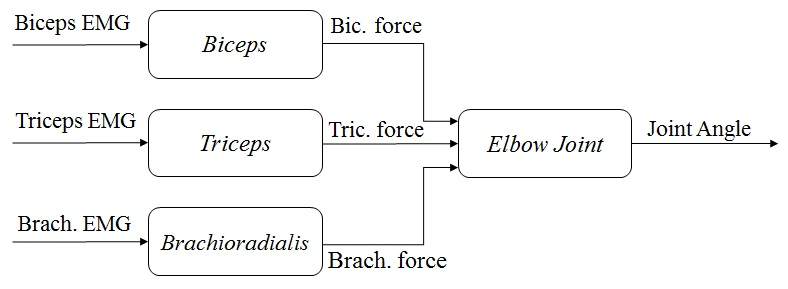
\includegraphics[width=0.98\columnwidth]{Images/Mechanical_Model.jpg}
      \caption{Model of the Muscle-Joint system}
      \label{ModelMuscle-Joint}
   \end{figure}

It is important to note that human models are complex and nonlinear \cite{kato2015}. One considerable advantage of using system identification as estimation technique is that it is possible to model the system as a black box. This allows the model estimation to be calculated without precise knowledge about muscles and joint dynamics \cite{Abbasi-Asl2011}. The estimation procedure proposed in this paper must be able to predict nonlinearities both on the input signals, since EMG signal presents nonlinearities, and output signals, because the movement of the elbow joint also has nonlinearities (e.g. arm movement is affected by gravity force). Considering these characteristics, the Hammerstein-Wiener model is a potential candidate for EMG-to-angle model estimation, since it is capable of estimating models from a black-box structure and predicting nonlinearities on both input and output signals. The Hammerstein-Wiener models have been previously used to estimate joint torque using EMG signals \cite{Abbasi-Asl2011,sab2010,clancy2012}. To our knowledge, no other authors used Hammerstein-Wiener models to estimate joint angle using EMG signals. We performed a search at Scopus.com using the terms ("EMG" OR "Electromyography") AND "Hammerstein-Wiener" in "All Fields". The results showed works containing parameter identification and the previously mentioned EMG to muscle force modeling.

The goal of this manuscript is to present the results of using Hammerstein-Wiener models to estimate the elbow joint angle, using the sEMG signals from biceps brachii, triceps brachii and brachioradialis, acquired through an experiment, as inputs to the system.

The paper is organized as follows: Section II presents the methods for experimentation, the experimental protocol and the recorded data processing. Section III explains the system modeling and mathematical analysis of the model. Section IV shows the results obtained that are discussed in Section V along with future research to continue this work.

\section{Methods}
\subsection{Subjects and experimental setup}
Two volunteers (age: 21 and 22 years, height: 1.92 m and 1.76 m, weight: 90 kg and 76 kg, both male, both right-handed) without known neuromuscular deficit participated in the experiments. The angle of the elbow joint as well as the surface Electromyography (sEMG) of three right arm muscles (biceps brachii,  triceps brachii and brachioradialis) were recorded. 
sEMG was measured with 3 pairs of BTS FREEEMG 1000 (BTS Spa, Italy) electrodes with an electrode separation of 20mm with the electrode diameter being 4mm. A pair of electrodes was placed on the biceps and other pair on the triceps following the SENIAM guidelines \cite{SENIAM20170110}. To determine the electrode positions of the brachioradialis muscle, the subject was asked to apply force to flex the forearm while keeping it at \(90^{\circ}\). Then, the electrodes were placed on the muscle belly separated by 20mm following the muscle fiber direction. The sampling rate was of 1kHz with 16 bit resolution. The user interface was the BTS FREEEMG software.

An Inertial Measurement Unit (IMU, VN-100 from VectorNav, TX, USA), with six degrees of freedom and \(0.01^{\circ}\) precision, was used to measure the joint angle during the movement. The angle data was acquired with an acquisition rate of 100 samples/second, using Matlab\textsuperscript{\textregistered} (The Mathworks Inc, USA) as the software for data acquisition and storage.


\subsection{Experimental Protocol}

\begin{figure}[thpb]
\vspace{3mm}
      \centering
      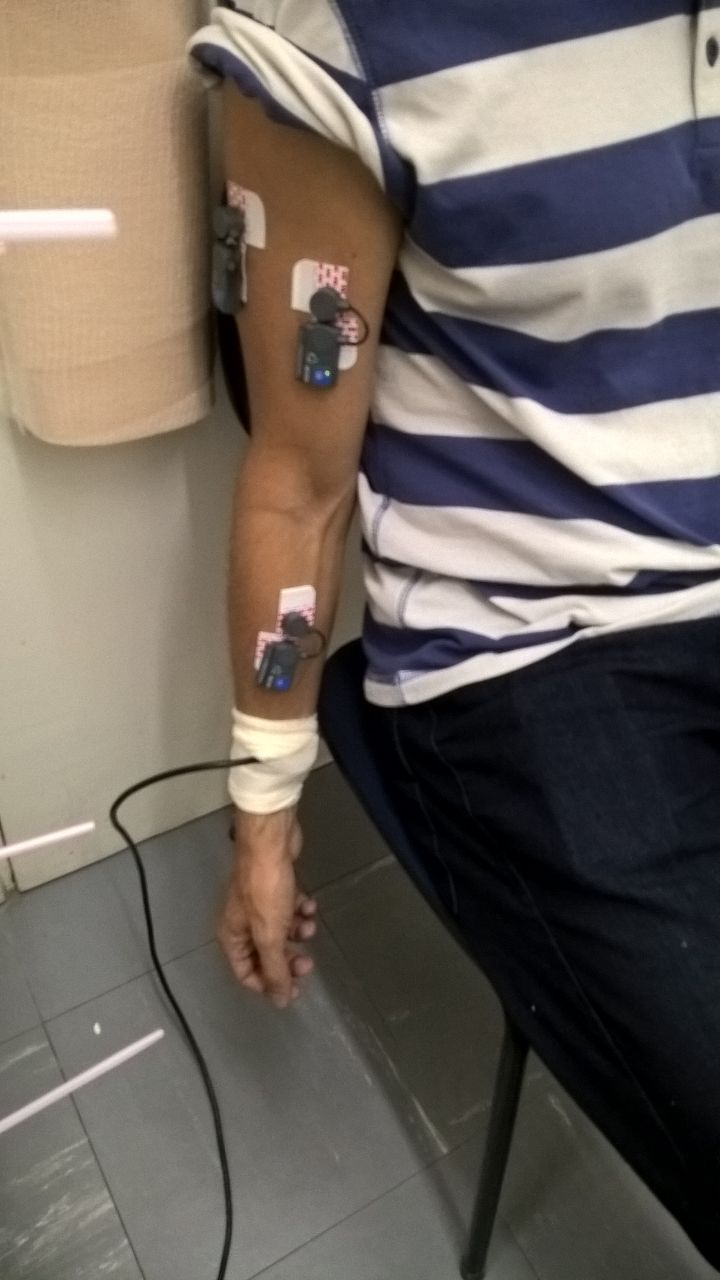
\includegraphics[scale=0.32]{Images/Experiment_Image.jpg}
      \caption{Experimental setup on a test subject}
      \label{Experimental Setup}
   \end{figure}

The subject sat on a chair, with both knees flexed at \(90^{\circ}\), with the back at a normal angle in relation to the ground, pressing the scapulae against the wall.

%The subject sat on a chair, with the knees flexed at \(90^{\circ}\), the back perpendicular to the ground with the scapulae pressed against the wall. The posterior part of the upper arm was leaning against a rubber support attached to the wall. This setup guaranteed that the subject was comfortable enough to perform repeated elbow flexions and extensions while maintaining the upper arm steady. 

The experimental protocol had three parts: The first one consisted of an isometric force test to obtain the Maximum Voluntary Contraction (MVC). The elbow of the subject was kept in a fixed position at \(90^{\circ}\) and he was asked to apply the maximal possible flexion force. Then, the participant was given a three minute interval before the next set.

In the second part, the subject should perform five continuous elbow flexions and extensions with an angular range from  \(50^{\circ}\) to \(140^{\circ}\) with a frequency of movement of 0.5Hz. To make the task easier for the subject, there was a template attached parallel to the subject's arm, providing visual guidance. A metronome, set at the speed of 60 beats per minute, allowed the subject to synchronize his movement with the sound. A minute of rest was given to the subject between each part.

In the third and final part of the experiment, the subject was asked to make a flexion movement of the elbow for 1 second, hold his arm at \(140^{\circ}\) for 1 s, followed by an extension movement for 1 s and then hold his forearm at \(50^{\circ}\) for 1 s. This movement should be repeated 5 times with no interval. Another one minute of rest was given to the test subject. The continuous and intermittent tests were repeated with 1.5kg and 3kg extra weight placed at the subject's hand.

The test was repeated in a different day, with both test subjects.

The experimental data (EMG and IMU) were transferred to Matlab\textsuperscript{\textregistered} for analysis and processing.


\subsection{Experimental Data Processing}

The EMG data were processed following procedures described in \cite{Rose20161112,Hayashibe20091621}.
\begin{enumerate}
\item High-pass filtering of the EMG data, using a 2nd order Butterworth filter, with a cutoff frequency of 30 Hz, removing movement artifact.
\item Full-wave rectification
\item Second Order Butterworth Filter, with 1 Hz cutoff frequency, obtaining the amplitude of the EMG signal.
\item normalization with the MVC peak.
\end{enumerate}

After this processing, the EMG signal is smoothed and presented as a percentage of the subject MVC.

A low-pass, 20 Hz cutoff frequency, second-order Butterworth filter was applied to the angular data to remove errors and other undesired signals.

It was necessary to resample, through interpolation, the position tracking data to 1 kHz, since it was acquired at a sampling rate of 100 Hz while the EMG data was acquired at a sampling rate of 1 kHz. 

Figure \ref{Angle and EMG} shows an example of the recorded elbow angle and processed sEMG for the continuous movement with no extra weight.




\section{System Modeling}

The chosen modeling technique to estimate the elbow joint angle using the EMG data as input was the Hammerstein-Wiener model. The structure of the Hammerstein-Wiener model can be seen in fig. \ref{HWmodel}. 

\begin{figure}[h]
      \centering
      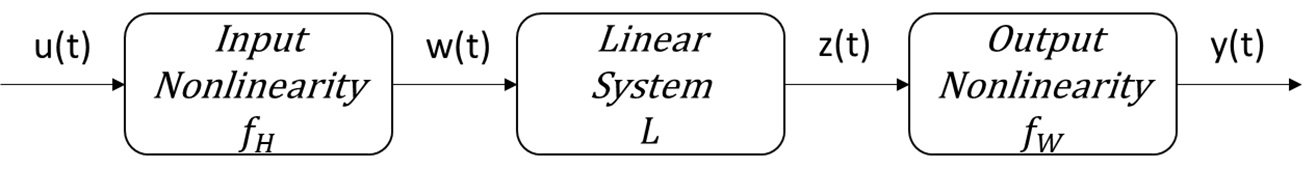
\includegraphics[width=0.98\columnwidth]{Images/HWmodel.jpg}
      \caption{Hammerstein-Wiener model structure}
      \label{HWmodel}
   \end{figure}

\begin{figure}[thpb]
\vspace{2mm}
      \centering
      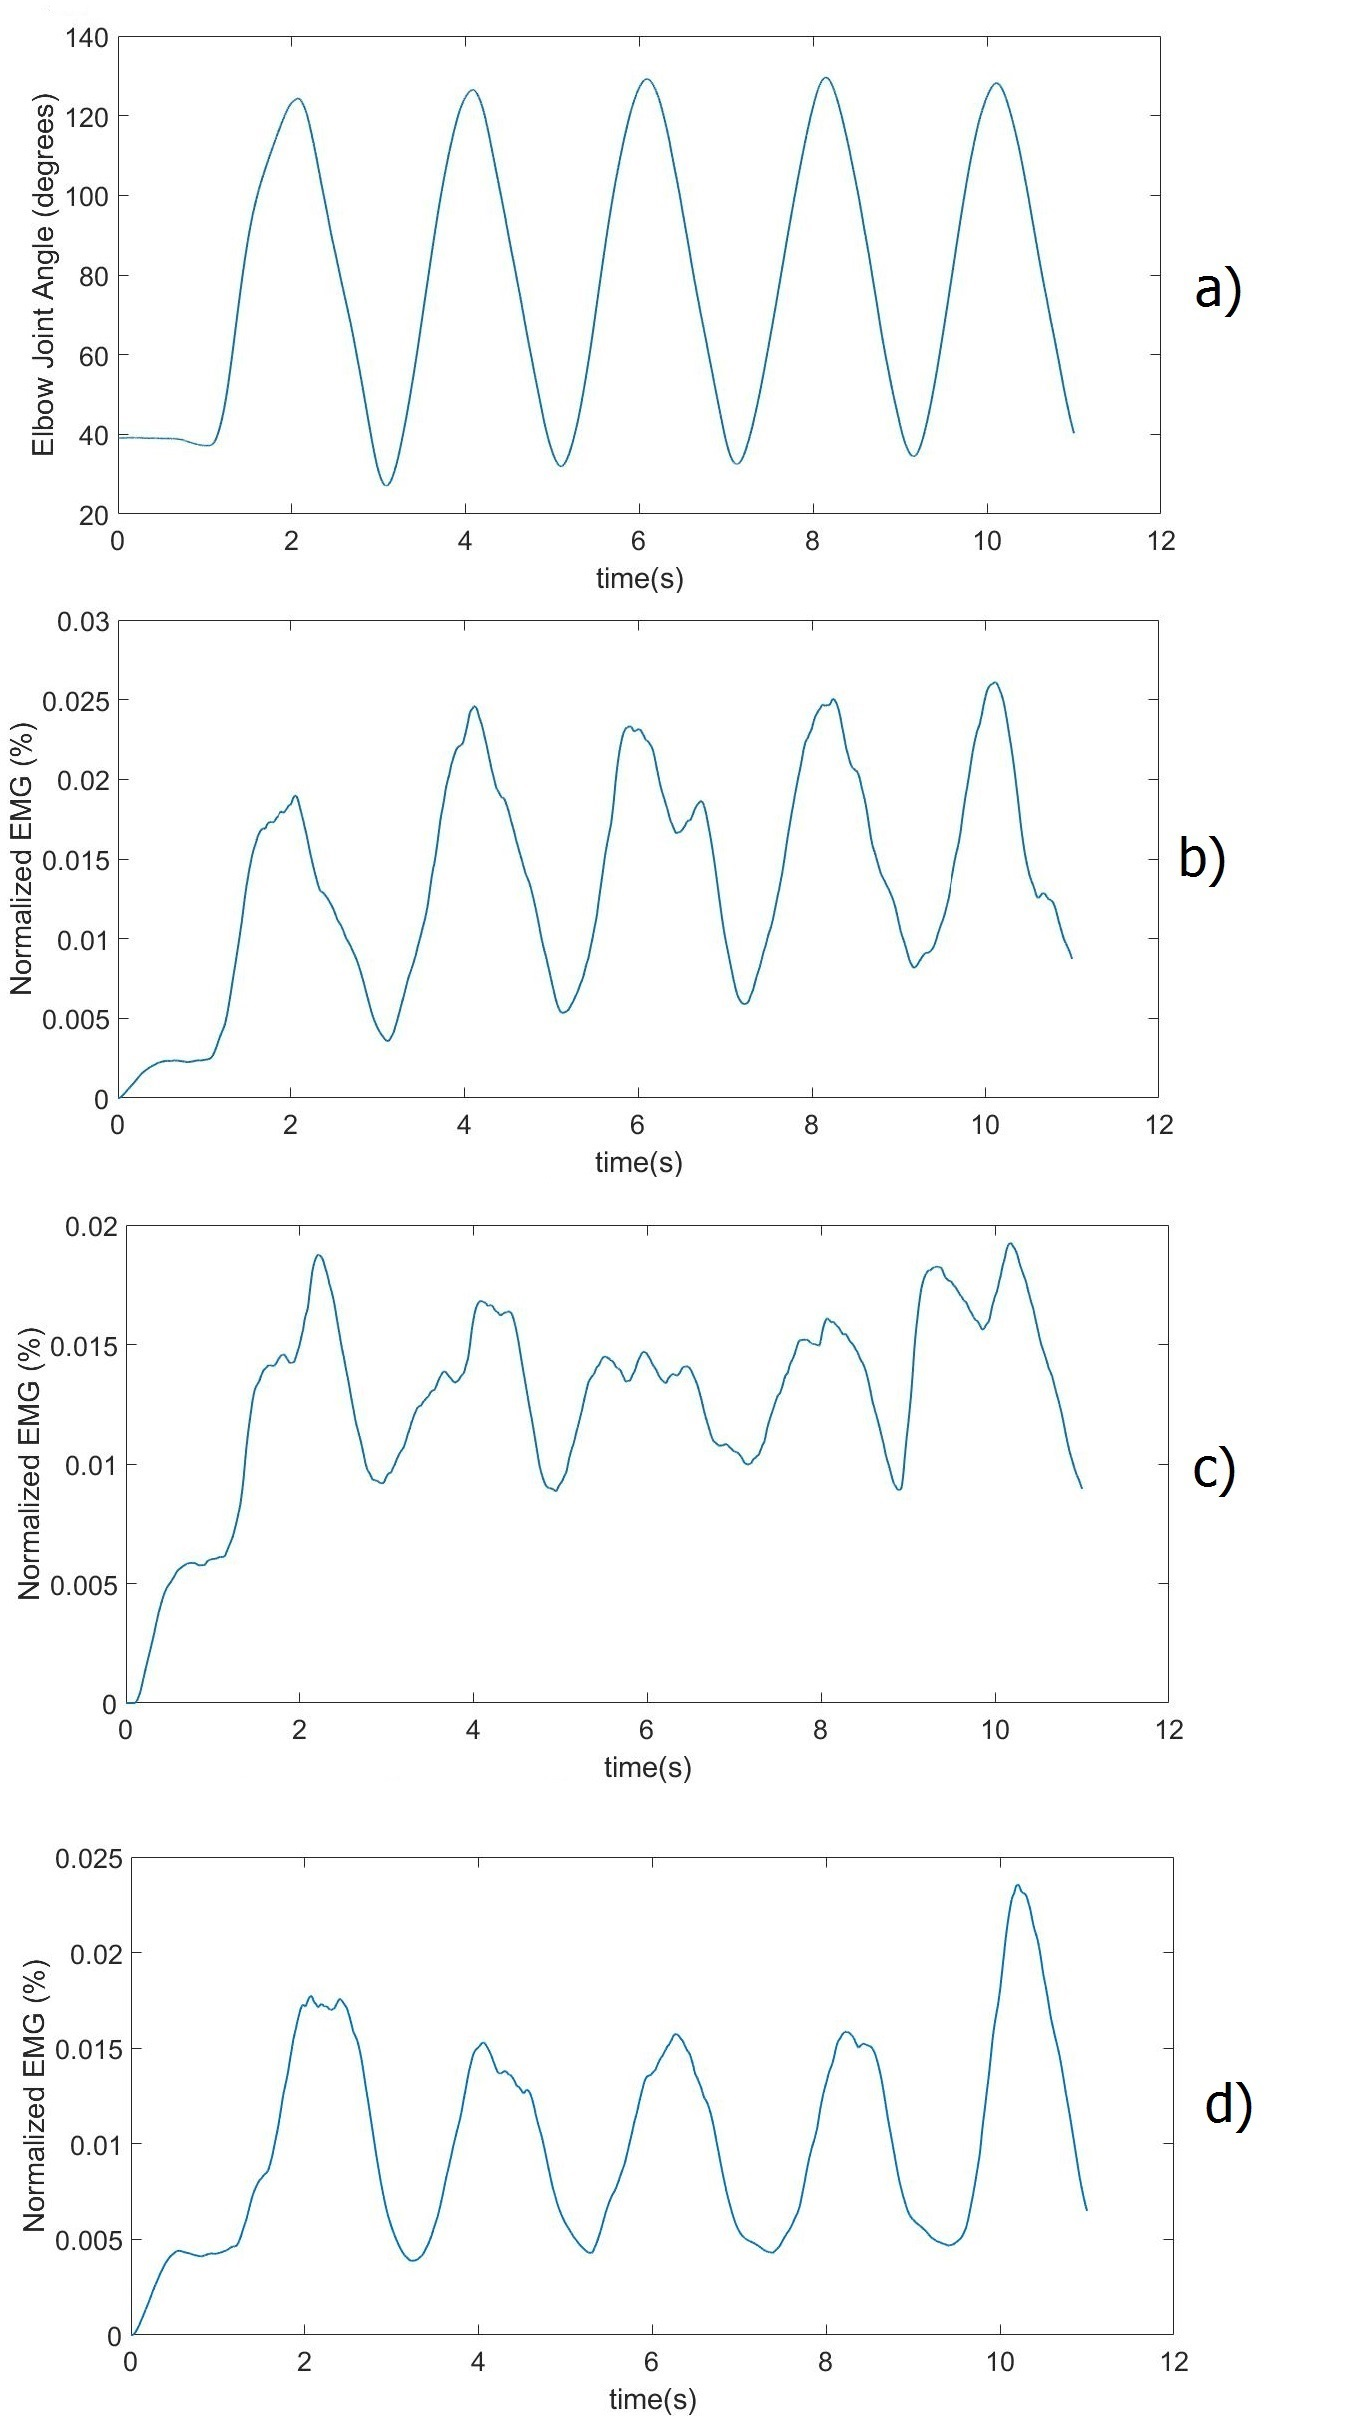
\includegraphics[width=0.98\columnwidth]{Images/Angle_and_EMGs.jpg}
      \caption{a) Joint angle for the continuous movement with no extra weight, recorded with the IMU; sEMG values for the b) biceps brachii, c) triceps brachii and d) brachioradialis for the continuous movement with no extra weight. }
      \label{Angle and EMG}
   \end{figure}

The Hammerstein-Wiener model is a block-oriented model, consisting of a composition of a linear dynamic block and nonlinear memoryless blocks \cite{Wills2013}. This model structure can be expressed as

\begin{equation}
\label{eq:yt}
y(t) = f_W(z(t))
\end{equation}

\begin{equation}
\label{eq:zt}
z(t) = L(w(t)) = \frac{B}{F}w(t)
\end{equation}

\begin{equation}
\label{eq:wt}
w(t) = f_H(u(t))
\end{equation}

Here, \(f_H(\cdot)\) is the input nonlinearity, \(f_W(\cdot)\) is the output nonlinearity, \(L(\cdot)\) is the Linear Time-Invariant system, \(\frac{B}{F}\) is a transfer function, \(t\) is the time variable, \(u(t)\) are the inputs, \(y(t)\) is the output, \(w(t)\) and \(z(t)\) are internal variables.

\(f_H\) and \(f_W\) are memoryless nonlinearities, i.e. static functions where the output value at time \(t\) depends only on input value at time \(t\). %For this estimation, wavelet networks were used as nonlinearities for both input and output.

Since the system being estimated is a MISO system the linear block is a transfer function vector in the form

\begin{equation}
\label{eq:B/F}
\frac{B_i(q)}{F_i(q)}
\end{equation}

Where \(i=1,2,3\) and \(q\) is the delay operator, representing the delay in time for each input to the system.

To determine the system, the orders of the numerator \(n_b\) and denominator \(n_f\) of the transfer function, as well as the input delays \(n_k\), must be specified.

In order to find a solution a search was done using 1000 models with random orders ranging from 1 to 15, with the following input and output nonlinearities: sigmoid network, wavelet network, piecewise linear function and one-dimensional polynomial. A window of 6s from the data vector was used to calibrate the model, while the entire data vector was used to validate the estimated model.

Each model was compared to the reference angle using equation \ref{eq:fitness}. The model orders that achieved the highest fitness value from this equation were chosen. The parameters of the models were estimated using time-domain data in Matlab\textsuperscript{\textregistered} (The Mathworks Inc, USA).

% With the model estimation technique chosen, it is necessary to determine the order of its parameters. To determine the chosen model order, 400 random combinations were tested for each data set with order values going from 0 to 10. The order chosen was the one that gave the best fit (see eq. \ref{eq:NRMSE}) between the calculated value and the one measured by the experiment. The coefficients of the models were estimated using time-domain data in Matlab\textsuperscript{\textregistered} (The Mathworks Inc, USA), minimizing a quadratic prediction error criterion.

\begin{equation}
\label{eq:fitness}
Fit = \sqrt[]{\frac{\prod_{i=1}^{3}\prod_{j=1}^{2} Corr_{ij}}{\sum_{i=1}^{3}\sum_{j=1}^{2} RMSE_{ij}}}
\end{equation}

Where $Corr_{ij}$ is the correlation between the measured angle and estimated angle for each test; $RMSE_{ij}$ is the Root-Mean-Square Error between the measured angle and estimated angle (see eq. \ref{eq:RMSE}); $i$ equals 1 for the 0kg test, 2 for the 1.5kg test and 3 for the 3kg test; j equals 1 for the continuous test and 2 for the intermittent test.

\begin{equation}
\label{eq:RMSE}
RMSE = \sqrt[]{mean((y-\hat{y})^2)}
\end{equation}

%\begin{equation}
%\label{eq:RMSE}
%NRMSE = 100*\left(1- \frac{||y-\hat{y}||}{||y-mean(y)||}\right)
%\end{equation}

Where $y$ is the measured angle and $\hat{y}$ is the estimated angle.

The coefficient of determination $R^2$ was also used to measure the fitness of the proposed model.

\begin{equation}
\label{eq:coeffDet}
R^2 = 1 - \frac{SS_{res}}{SS_{tot}}
\end{equation}

Where

\begin{equation}
\label{eq:SSres}
SS_{res} = \sum_{i=1}(y_i-\hat{y_i})^2
\end{equation}

\begin{equation}
\label{eq:SStot}
SS_{tot} = \sum_{i=1}(y_i-\bar{y})^2
\end{equation}

\begin{equation}
\label{eq:bary}
\bar{y} = \frac{1}{n} \sum_{i=1}^{n} y_i
\end{equation}

Where $\bar{y}$ is the mean value of the measured angles.

% Adicionar parágrafo: The coefficient of determination was also used to test the fitness of the proposed model. Inserir equação do coefi

% The chosen method for the modeling of the relationship between elbow joint angle and sEMG was a system identification method called Auto Regressive Moving Average with Exogenous Input (ARMAX). The ARMAX model has the following form:

% For each model, the data acquired from each test subject was separated by weight lifted and the data from the continuous movement and the intermittent movement were merged. This way, it was possible to calculate a single model for the arm movement using the system identification tool in Matlab\textsuperscript{\textregistered}.



%------------Paragrafo AIC---------------------

%In order to find a solution a search was done using 1000 models with random orders ranging from 1 to 7. The chosen model orders were the ones that minimized the Akaike Information Criteria (AIC) index.

%Since we estimated three different models, one for each different weight being carried, three different values for the AIC index were obtained. To determine the model orders that, overall, minimized the AIC index, we used eq. \ref{eq:aic}

%\begin{equation}
%\label{eq:aic}
%Fit = \sqrt[]{\sum_{i=1}^{3}AIC_i}
%\end{equation}

%Where \(AIC_i\) 


\section{Results}

The model orders calculated are presented in table \ref{ta:order}. Since the system is using three inputs, $n_b, n_f$ and $n_k$ are three dimensional. The input and output nonlinearity that achieved highest fitness values was the Wavelet Network.

\begin{table}[h]
\caption{Model orders for each subject}
\label{ta:order}
\centering
\begin{tabular}{|c|c|c|c|}
\hline
 & \(n_b\) & \(n_f\) & \(n_k\)\\
\hline \hline
Subject 1 & 4, 4, 0 & 9, 15, 0 & 12, 15, 0\\
\hline
Subject 2 & 7, 12, 15 & 2, 3, 14 & 11, 1, 11\\
\hline
\end{tabular}
\end{table}

\begin{figure}[thpb]
      \centering
      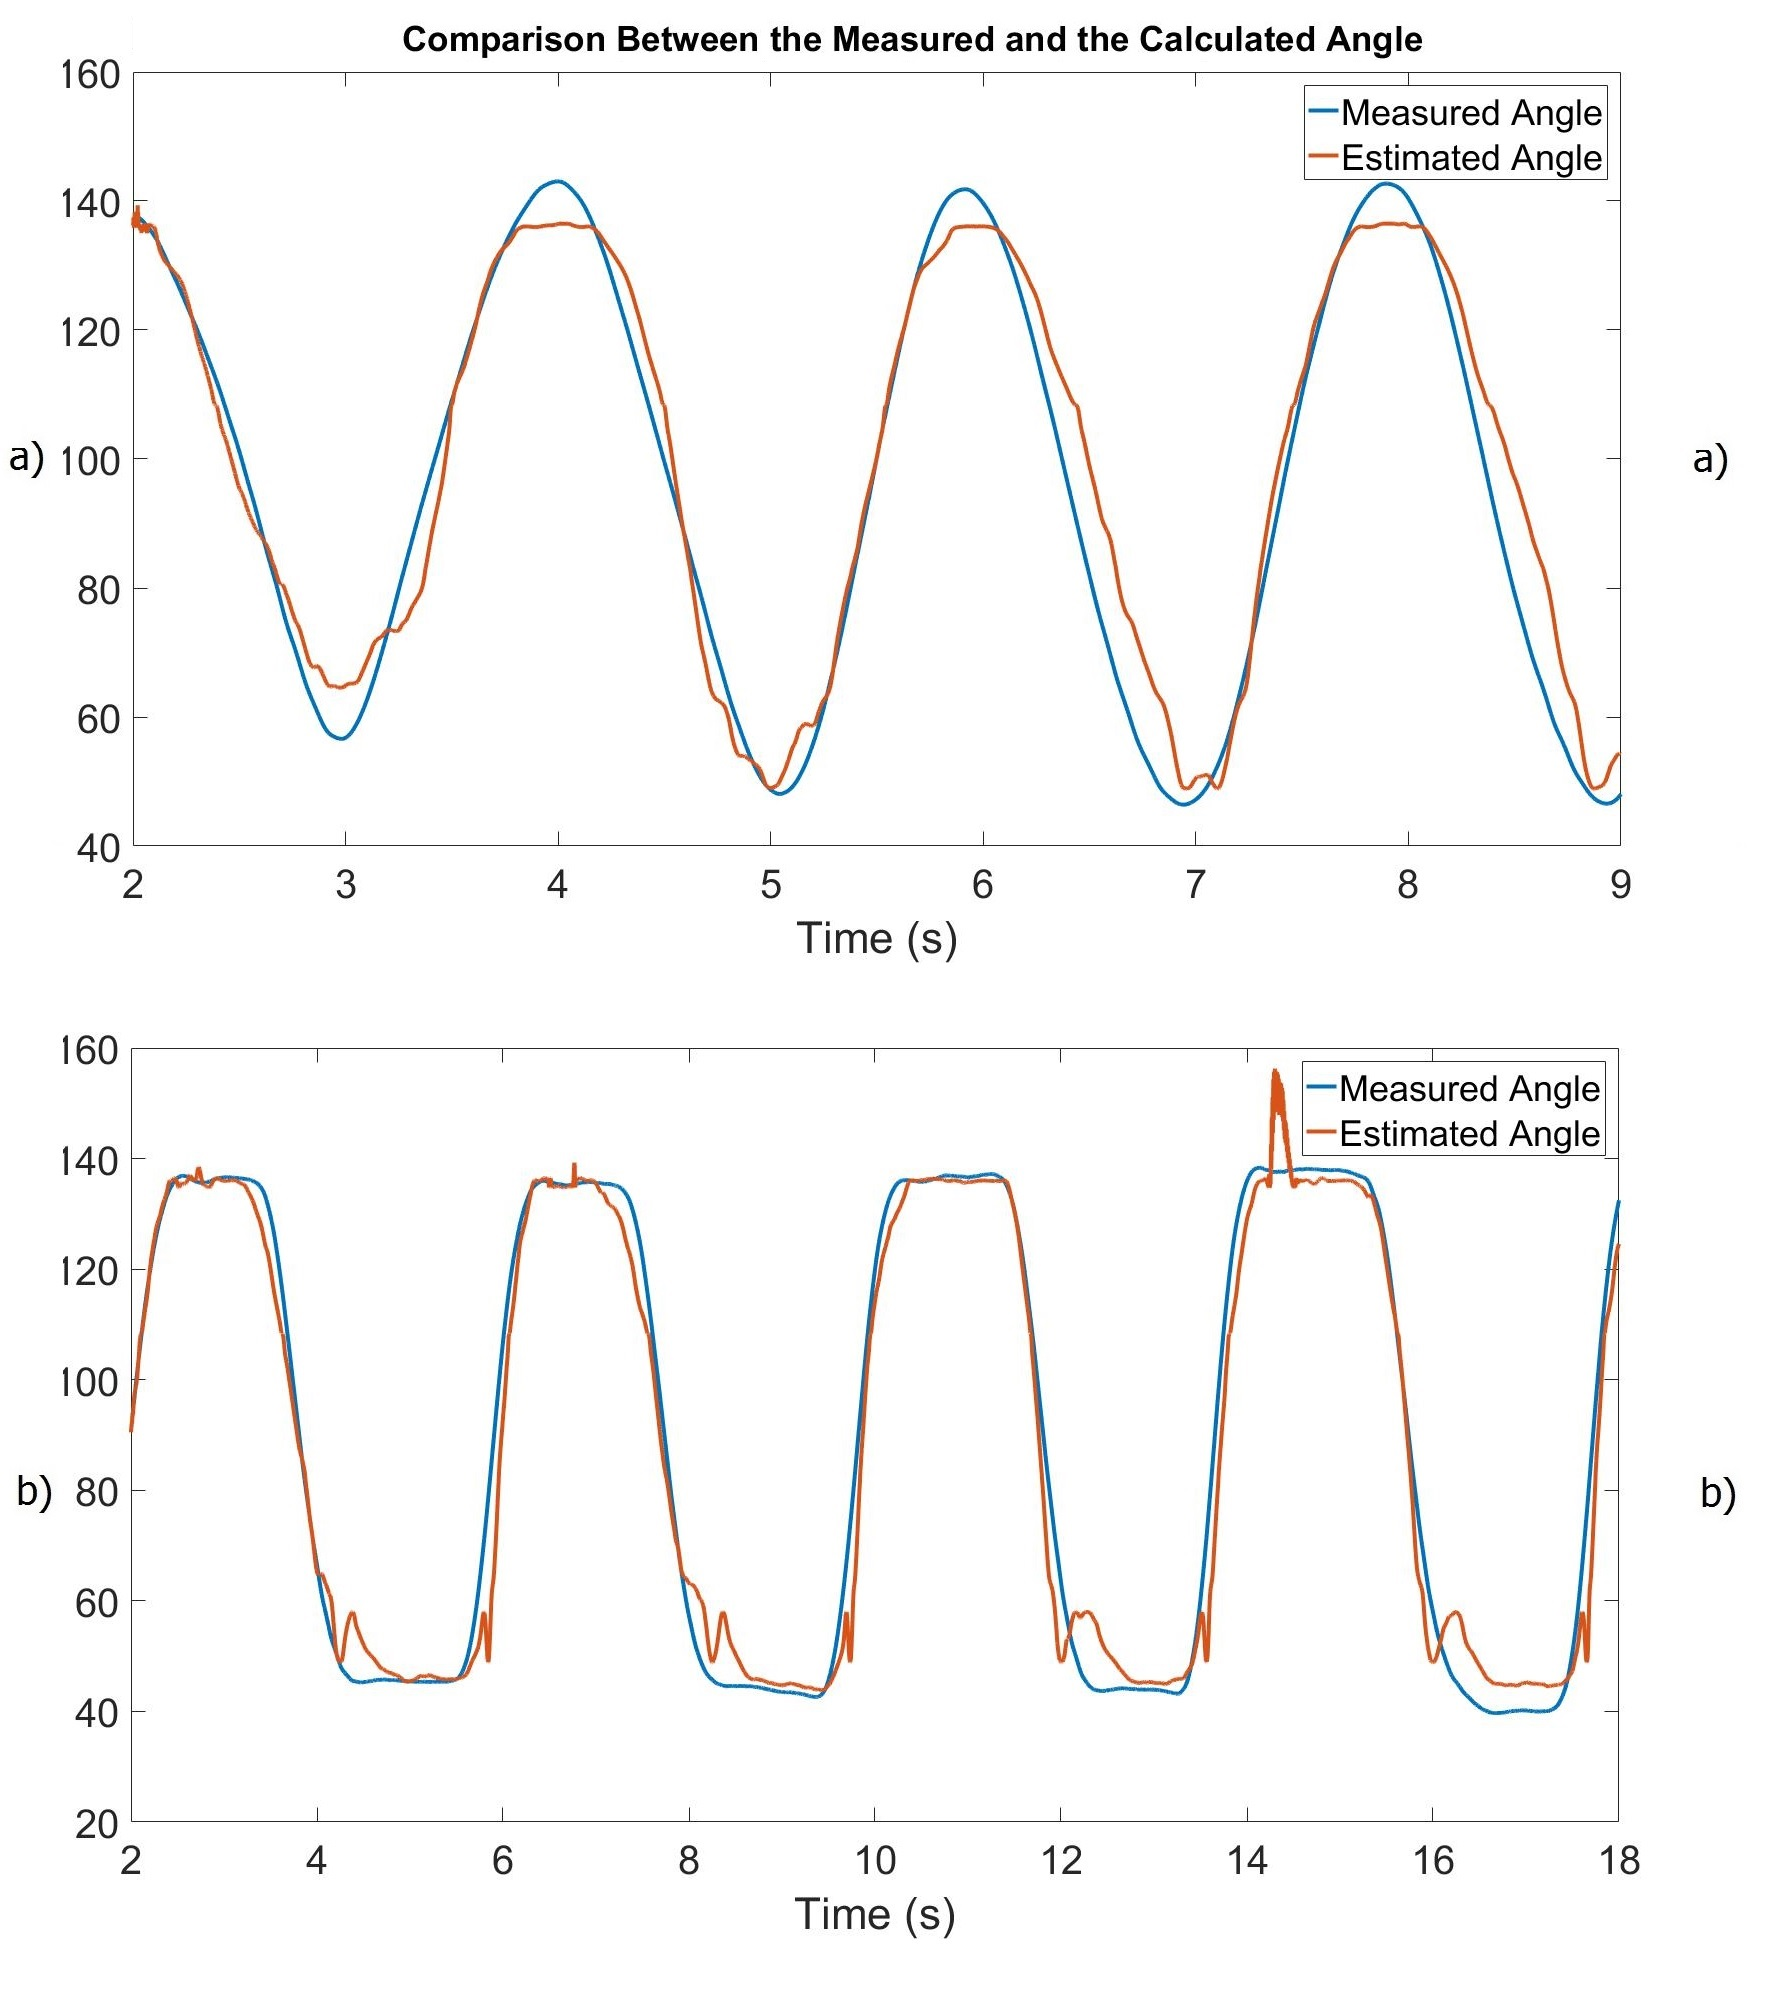
\includegraphics[width=0.98\columnwidth]{Images/comparison.jpg}
      \caption{Comparison between the measured angle of the elbow joint and the angle calculated through the use of the estimated model, for subject 1, with a 1.5kg dumbbell. a) shows the comparison for the continuous movement and b) the comparison for the intermittent movement}
      \label{Angle Comparison}
   \end{figure}
   
   \begin{table*}[h]
   \vspace{2mm}
\caption{Correlation factor, coefficient of determination and Root-mean-square error for the calculated and measured angle values}
\label{ta:correlation}
\centering
\resizebox{0.99\textwidth}{!}{%
\begin{tabular}{|c c|c c c|c c c|c c c|c c c|c c c|c c c|}
\hline
\multicolumn{2}{|c|}{} & \multicolumn{6}{c|}{Model Estimation, first test set} & \multicolumn{6}{c|}{Same model, second test set} & \multicolumn{6}{c|}{New model, same orders, second test set} \\
\hline
\multicolumn{2}{|c|}{} & \multicolumn{3}{c|}{Continuous} & \multicolumn{3}{c|}{Intermittent} & \multicolumn{3}{c|}{Continuous} & \multicolumn{3}{c|}{Intermittent} & \multicolumn{3}{c|}{Continuous} & \multicolumn{3}{c|}{Intermittent} \\
\hline
\multicolumn{2}{|c|}{} & Correlation & $R^2$ & RMSE & Correlation & $R^2$ & RMSE & Correlation & $R^2$ & RMSE & Correlation & $R^2$ & RMSE & Correlation & $R^2$ & RMSE & Correlation & $R^2$ & RMSE\\
\hline \hline

& 0 kg &0.9623 & 0.9232 & 9.394 &0.9624 & 0.8932 &12.91 & 0.8780 & 0.5114 & 17.86 & 0.9697 & 0.9205 & 9.647 &0.9525 & 0.9044 &7.898 & 0.9708 & 0.8602 &12.79\\
Subject 1 & 1.5 kg &0.9780 & 0.9480 &7.390 &0.9865 & 0.9714 & 6.846 &0.9129 & 0.7403 &14.21 & 0.9666 & 0.9339 & 8.870 &0.9169 & 0.8400 &11.15 &0.9328 & 0.8470 &13.50 \\
& 3 kg &0.9816 & 0.9499 &6.796 &0.9631 & 0.9200 &11.477 & 0.9330 & 0.8526 & 10.31 & 0.7956 & 0.6161 & 22.70 &0.9497 & 0.8912 &8.860 &0.9730 & 0.8923 &12.03\\
\hline

& 0 kg &0.9729 & 0.9440 &7.662 &0.9620 & 0.9244 &10.10 & 0.8825 & 0.7669 & 16.44 & 0.9330 & 0.8657 & 13.98 &0.9787 & 0.9570 &7.062 &0.9620 & 0.9099 &11.45\\
Subject 2 & 1.5 kg &0.9596 & 0.9202 &8.9476 &0.9493 & 0.8859 & 11.62 & 0.9754 & 0.9425 & 7.927 & 0.9413 & 0.8683 & 14.09 &0.9838 & 0.9673 &5.976 &0.9211 & 0.8482 &15.12\\
& 3 kg &0.9788 & 0.9556 &6.733 &0.9808 & 0.9612 &6.540& 0.8767 & 0.7668 & 15.35 & 0.9625 & 0.9191 & 11.02 &0.9847 & 0.9688 &5.614 &0.9721 & 0.9431 &9.246\\
\hline

\end{tabular}%
}
\centering

\label{ta:corr}
\end{table*}

Using the values from table \ref{ta:order} as the Hammerstein-Wiener model orders, we estimated the model for elbow joint angle using the sEMG data as input and compared the results to the experimentally measured values. As an example, figure \ref{Angle Comparison} shows a comparison between the measured and estimated angle, for both continuous and intermittent movement, for subject 1.

Using the same model orders and parameters calculated previously, a second model estimation was performed using a second batch of data, recorded in a different day. An example of the result of this process is shown in figure \ref{Validation Procedure}, where the model calculated for subject 2 was used to estimate the elbow joint angle using the input data acquired from the second day of testing.

The data acquired from the second experimental set were also used to generate a new model, using the same model orders determined in first experimental set (table \ref{ta:order}). This way, it is possible to evaluate if the same orders determined in one experiment can be carried over to tests performed in a different experimental set.

   


To better determine the accuracy of the model, three performance parameters were used: the correlation coefficient, the determination coefficient and the Root-Mean-Square Error (RMSE) between the estimated and the measured elbow joint angles. Table \ref{ta:corr} shows the accuracy performance parameters for each participant and every test set. The different results for each method described above are presented in columns. First, using the first data set to estimate a model and comparing the result to the measured angle values; second, using the same model calculated for the first experimental set to estimate the angle, but using the data from the second experimental set as input to the model; and finally, using the same model orders chosen from the first experimental set, a new model was generated based on the second data set and comparing the output to the measured angle data.

The estimated models achieved correlation values of $94.90 \pm 3.92\%$, coefficient of determination of $0.8814 \pm 0.0978$ and RMSE values of $10.82 \pm 3.73^\circ$


\section{Discussion}

This paper proposed a method to estimate the elbow joint angle based on the measurement of the sEMG of biceps brachii, triceps brachii and brachioradialis from two test subjects. The sEMG-to-Angle model was estimated using the data collected from the experiments and a Hammerstein-Wiener model with Wavelet Network as input and output nonlinearities. With the acquired sEMG data as input to the estimated model, it was possible to estimate the elbow angle. Using the data from the IMU (real angle value) it was possible to validate the estimation based on sEMG.

\begin{figure}[bthp]
      \centering
      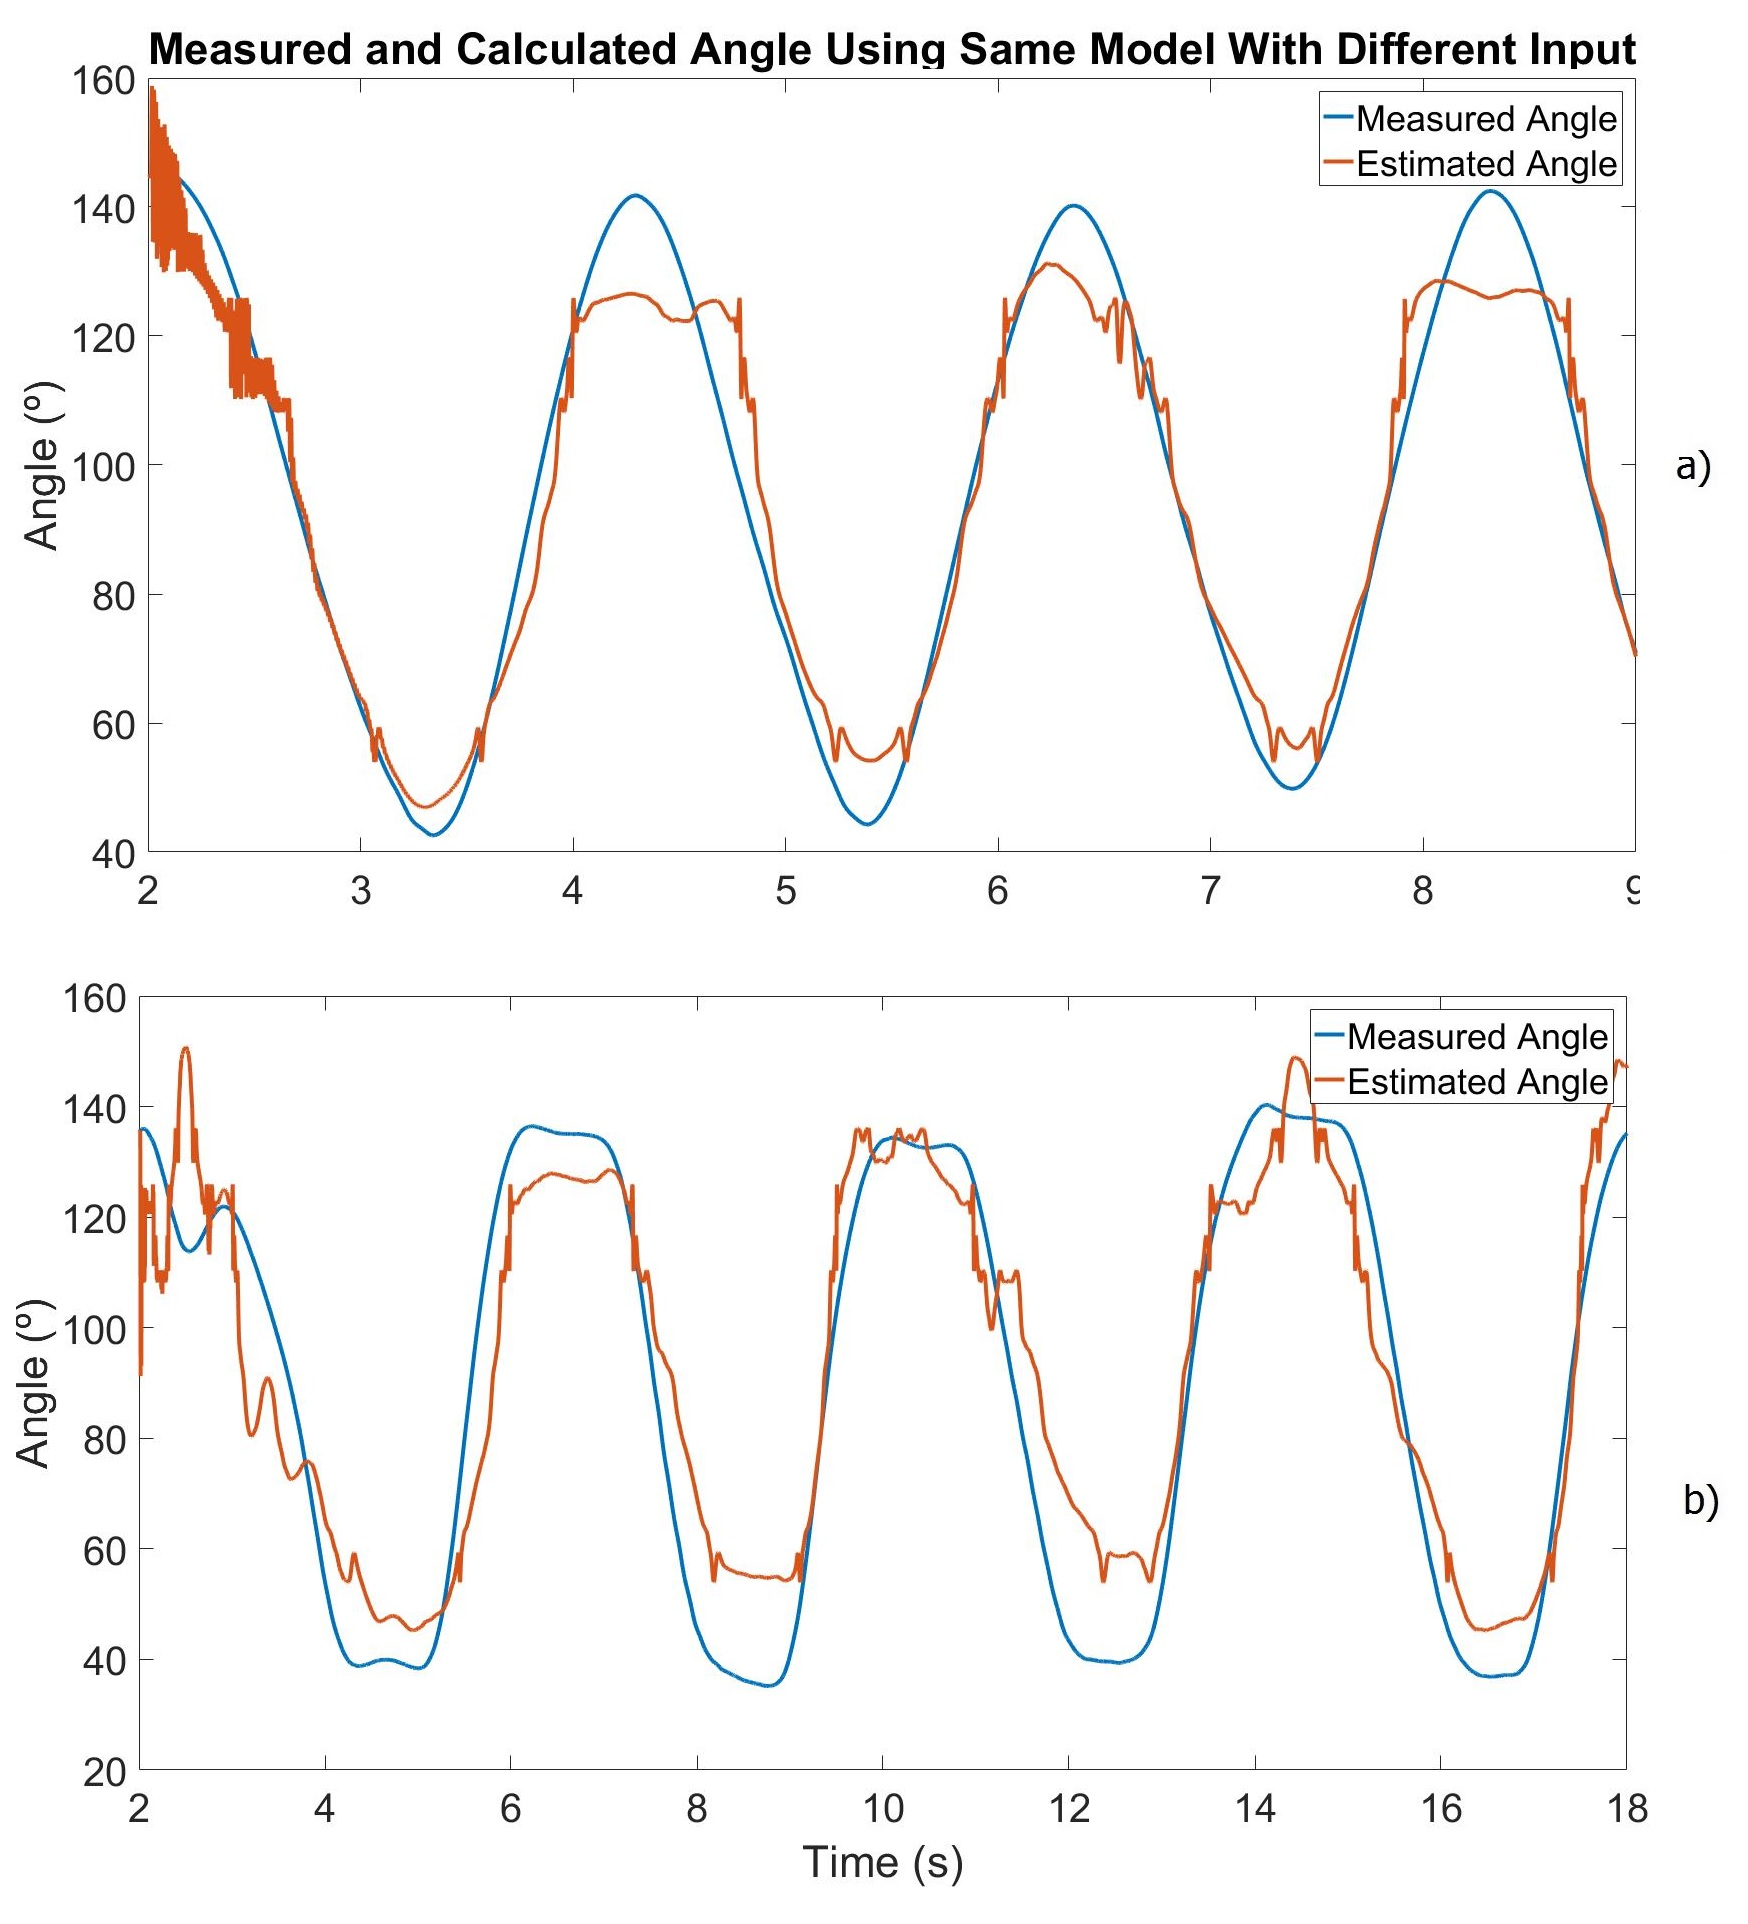
\includegraphics[width=0.95\columnwidth]{Images/Different_Input.jpg}
      \caption{Comparison of the estimated and measured joint angle using the same model calculated with the first data set, but using the EMG data from the second test set as input for subject 2 with a 1.5kg dumbbell. a) shows the comparison for the continuous movement and b) the comparison for the discrete movement}
      \label{Validation Procedure}
   \end{figure}

The experimental data showed that it is possible to use the EMG data to estimate the joint angle, with prior knowledge of the weight being lifted, at least for the experimental conditions performed during the tests.
%Even though estimating one model for continuous movement and another one for discrete movement gives higher precision, it is possible to calculate a single model for both movements.

\addtolength{\textheight}{-4cm}   % This command serves to balance the column lengths
                                  % on the last page of the document manually. It shortens
                                  % the textheight of the last page by a suitable amount.
                                  % This command does not take effect until the next page
                                  % so it should come on the page before the last. Make
                                  % sure that you do not shorten the textheight too much.



%%%%%%%%%%%%%%%%%%%%%%%%%%%%%%%%%%%%%%%%%%%%%%%%%%%%%%%%%%%%%%%%%%%%%%%%%%%%%%%%



%%%%%%%%%%%%%%%%%%%%%%%%%%%%%%%%%%%%%%%%%%%%%%%%%%%%%%%%%%%%%%%%%%%%%%%%%%%%%%%%



%%%%%%%%%%%%%%%%%%%%%%%%%%%%%%%%%%%%%%%%%%%%%%%%%%%%%%%%%%%%%%%%%%%%%%%%%%%%%%%%


%%%%%%%%%%%%%%%%%%%%%%%%%%%%%%%%%%%%%%%%%%%%%%%%%%%%%%%%%%%%%%%%%%%%%%%%%%%%%%%%


The results achieved with this procedure had similar precision values as reported by other authors using different methods \cite{Rahmatian2016158,Mamikoglu2016785,Pang2015165,Liu1999391}. Even though other authors used the Hammerstein-Wiener model to determine EMG-to-Muscle Force relation instead of a EMG-to-Angle relation, the results show similar precision values \cite{Abbasi-Asl2011,sab2010,clancy2012}
For the majority of simulations, the model achieved values of correlation over $90\%$, coefficient of determination over $0.9$ and RMSE under $15^\circ$.

%As stated before, by lifting different weights the model parameters are altered. For the same test subject the A(q) and C(q) parameters (see eq. 3) maintained values with less than 1\% difference from one another, while the B(q) values assumed a greater range of values.

%Even for different subjects, the estimated A(q) and C(q) parameters also had a difference of less than 1\% from one another.

%From the seven subjects, six of them could be estimated by an ARMAX model with the same parameters order. The test subject with different order parameters was the one that presented the worst readings of the brachioradialis muscle EMG. Because of that, a lot of noise is introduced, requiring a higher order system to overcome the modeling errors. The brachioradialis is the most difficult muscle to read the sEMG signals compared to the biceps brachii and the triceps brachii. This difficulty is due to the muscle short length causing the electrodes to stay close to the tendon, which induces  reading errors. Not coincidentally, this test subject was the one with smaller stature.

%The repeatability of the model was successful for the cases studied in this work, even though it is possible to note that the model is not as precise as it was for the calibration procedure.



For both subjects, in the worst case, correlation was above $79\%$, coefficient of determination above $0.5$ and RMSE below $23^\circ$. It is possible to note that the simulation results when using the same model for different data inputs are worse than the results presented when using the same data used for model calibration. Since the EMG signals may change between tests, due to slight changes in electrode position, tissue properties or temperature \cite{soderberg1975}, it may not be possible to determine a model capable of estimating the joint angle for data acquired on different days or test setups with the same quality of results. But even in this case, these results can be favorably compared to other similar works \cite{Rahmatian2016158,Mamikoglu2016785,Pang2015165,Liu1999391}. More investigation is required to determine if those models are capable of estimating the joint angle for any test conducted with these test subjects.

The same model orders calculated through the first experimental set can be used for other test sessions, without loss of accuracy. Even though environmental noise and other undesirable signals affect the EMG signal, it does not change the system order.

In future work, we will apply the techniques used in this work to a larger set of subjects. Also, we will further study the use of system identification, in two ways, one, assessing the possibility of a weight-independent model estimator and, second, the estimation of a subject-independent model. Real-time testing will be performed as these models will be used as part of an EMG-driven control system for exoskeletons.



\bibliography{biblio_EMG_Joint}
\bibliographystyle{unsrt}





\end{document}
